\documentclass[11pt]{article}
\usepackage[T1]{fontenc}
\usepackage{lmodern}
\usepackage[margin=1in]{geometry}
\usepackage{amsmath,amssymb,amsthm,mathtools}
\usepackage{booktabs,array,longtable}
\usepackage{xcolor,microtype,fancyhdr,enumitem}
\usepackage{tikz}
\usepackage[hyphens]{url}
\usepackage{xurl}
\usepackage[colorlinks=true,linkcolor=blue!45!black,citecolor=blue!45!black,urlcolor=blue!45!black,hypertexnames=false]{hyperref}
\usepackage{listings}
\setlist{itemsep=3pt,topsep=5pt}
\lstset{basicstyle=\ttfamily\footnotesize,breaklines=true,columns=fullflexible,keepspaces=true,frame=single,rulecolor=\color{black!15}}
\pagestyle{fancy}\fancyhf{}
\fancyhead[L]{\small Cauchy and residues in iPRA}
\fancyhead[R]{\small Finite quantitative proofs}
\fancyfoot[C]{\thepage}
\setlength{\headheight}{14pt}
\setlength{\emergencystretch}{2em}
\newtheorem{theorem}{Theorem}[section]
\newtheorem{lemma}[theorem]{Lemma}
\newtheorem{proposition}[theorem]{Proposition}
\newtheorem{corollary}[theorem]{Corollary}
\theoremstyle{definition}
\newtheorem{definition}[theorem]{Definition}
\newtheorem{remark}[theorem]{Remark}
\newcommand{\N}{\mathbb N}
\newcommand{\Z}{\mathbb Z}
\newcommand{\Q}{\mathbb Q}
\newcommand{\C}{\mathbb C}
\newcommand{\ipra}{\mathsf{iPRA}}
\newcommand{\norm}[1]{\left\lVert#1\right\rVert_1}
\newcommand{\abs}[1]{\left|#1\right|}
\newcommand{\eps}[1]{2^{-#1}}
\newcommand{\dd}{\,\mathrm d}
\newcommand{\Res}{\operatorname{Res}}
\newcommand{\Wind}{\operatorname{wind}}
\newcommand{\code}[1]{\texttt{#1}}
\newcommand{\trap}{\mathcal T}
\newcommand{\Int}{\mathcal I}
\newcommand{\bd}{\partial}
\title{Cauchy's integral theorem and the residue theorem\\in intuitionistic primitive recursive arithmetic}
\author{A constructive proof package prepared for Vladimir Reshetnikov}
\date{November 15, 2026}
\hypersetup{pdftitle={Cauchy's integral theorem and the residue theorem in iPRA},pdfauthor={Prepared for Vladimir Reshetnikov},pdfsubject={Complete quantitative human-readable proofs and a Lean formalization roadmap},pdfkeywords={iPRA, constructive complex analysis, Cauchy integral theorem, residue theorem, Laurent series, primitive recursion}}
\begin{document}
\maketitle
\begin{abstract}
We prove effective, quantitative versions of Cauchy's integral theorem and
the residue theorem using intuitionistic first-order arithmetic with
primitive-recursive function symbols and quantifier-free induction.
Complex numbers are represented by rational approximation procedures;
uniform continuity, uniform first-order differentiability, separation,
and geometric data are explicit inputs. Every analytic equality abbreviates
a family of finite rational estimates with primitive-recursive precision
bounds.

The central Cauchy estimate comes from four-way triangle subdivision,
exact cancellation of internal trapezoidal sums, and exact annihilation of
complex-affine functions. We compute the exceptional square moment
\(\oint (z-a)^{-1}\dd z=2\pi i\) from rational real-variable sums.
We then prove an annular Cauchy formula and derive, rather than assume,
uniformly convergent Laurent approximations with an explicit geometric
tail. A finite planar filling gives the residue formula, including isolated
essential singularities. Supplied quantitative curve and homotopy data
also permit an extension beyond polygons.

The result is a theorem schema in fixed primitive-recursive input
procedures, not an assertion that arbitrary classical functions are
objects of first-order arithmetic. The mathematical proofs are complete
for the stated effective hypotheses. The accompanying Lean source is an
uncompiled finite algebra candidate; the detailed roadmap specifies the
remaining work needed to construct deeply embedded iPRA derivations in
ProveIt's ConciseIPRA library. No completed Lean formalization is claimed.
\end{abstract}
\newpage
\begingroup
\footnotesize
\tableofcontents
\endgroup
\newpage

\section{The results and their scope}\label{sec:scope}

The familiar conclusions are
\begin{equation}\label{eq:maincauchy}
 \oint_\Gamma f(z)\dd z=0
\end{equation}
when the cycle has a filling on which \(f\) is holomorphic, and
\begin{equation}\label{eq:mainresidue}
 \oint_\Gamma f(z)\dd z
   =2\pi i\sum_{j=1}^{J}\Wind(\Gamma,a_j)\Res(f,a_j)
\end{equation}
in the presence of finitely many isolated singularities. These are the
homological forms of the theorems requested in the problem
\cite{wikicauchy,wikiresidue}. The precise effective readings proved here
are as follows.

\begin{theorem}[Effective Cauchy theorem, preview]\label{thm:previewc}
Fix primitive-recursive rational approximation procedures for \(f\) and a
complex derivative coefficient, together with the continuity and
first-order remainder moduli of Section~\ref{sec:data}. Let \(T\) be a
finite rational oriented triangle chain, with all its triangles in the
certified carrier of these data. Then \(\Int_{\bd T}(f)=0\).
At every requested precision there is an explicit primitive-recursive
mesh and sample precision for which the corresponding rational contour
sum has norm at most the requested dyadic error.
\end{theorem}

\begin{theorem}[Effective residue theorem, preview]\label{thm:previewr}
Let \(\Gamma\) be a finite closed rational polygonal integer chain, and
let \(a_1,\ldots,a_J\in\Q(i)\) be pairwise separated singularity centres.
Give positive rational radii \(r_j\), disjoint local outer squares
\(Q_{8r_j}(a_j)\) avoiding \(\Gamma\), and a rational triangle chain with
\begin{equation}\label{eq:certificate}
 \bd T=\Gamma-\sum_{j=1}^{J}w_j\bd Q_{r_j}(a_j).
\end{equation}
The carrier of \(T\) has a supplied positive rational clearance from
each centre. Supply effective holomorphy data
on this carrier and on the local annuli
\(Q_{8r_j}(a_j)\setminus\operatorname{int}Q_{r_j/8}(a_j)\).
Then the local Laurent coefficient \(a_{j,-1}\) can be constructed
primitive recursively, and
\[
 \Int_\Gamma(f)=2\pi i\sum_jw_j a_{j,-1}.
\]
These coefficients are unique Laurent coefficients and the integers
\(w_j\) are intrinsic winding indices. For a function presented on a
punctured neighbourhood, the coefficient is independent of the chosen
admissible local radii and is its residue.
\end{theorem}

The annular hypotheses in the second theorem suffice for the displayed
identity. To speak of an isolated singularity of an entire punctured germ,
the same evaluator is given on the punctured neighbourhood, with
primitive-recursive bounds and moduli on its closed rational annuli.
No finite pole order is assumed. The annular theorem itself does not
assert that a function specified only on one annulus extends to the
punctured disc.

Equation~\eqref{eq:certificate} is a finite geometric witness, not an
assumption about the value of the desired integral.
Section~\ref{sec:geometry} constructs it by rational planar subdivision
and crossing counts. For a general open domain one must also certify that
the resulting nonzero-weight triangles are in that domain. In a convex
domain, ordinary fan triangles suffice for Cauchy's theorem. We give a
separate extension to curves with supplied variation and continuity data
in Section~\ref{sec:curves}.

\paragraph{What is, and is not, a hypothesis.}
The data include approximation routines, positive separation bounds,
and uniform moduli. They do not include Cauchy's theorem, the residue
identity, a Laurent expansion, Jordan separation, or a classical
compactness theorem. Bare pointwise complex differentiability is not
silently converted into a primitive-recursive uniform modulus.
The rational-centre, polygonal statement is the core theorem; more
general curves are covered under the additional explicit data stated
later. No unrestricted theorem about every set-theoretic complex function
is being asserted inside first-order arithmetic.

Constructive complex analysis has a substantial prior development.
Bridges proves a homotopy form of Cauchy's theorem in Bishop-style
constructive mathematics \cite{bridges}. That framework includes a
type- or set-theoretic background beyond the present first-order theory.
Here the additional work is to expose finite estimates and their
primitive-recursive bounds, and to account for the permitted induction.

\section{The arithmetic foundation and representations}\label{sec:foundation}

\subsection{The theory and the meaning of a theorem schema}

Use intuitionistic first-order logic with equality, zero, successor, a
symbol for each primitive-recursive function, their defining equations,
successor separation and injectivity, and induction for quantifier-free
formulas with numerical parameters. This is the presentation
\code{PRAAx} in ProveIt's \code{ConciseIPRA/PR.lean} \cite{prsource}.
The actual derivability relation in that library is used in
Section~\ref{sec:lean}; an ambient Lean theorem about \(\C\) would have a
different meaning.

Each occurrence of an input procedure such as \(F(z,n)\), a modulus
\(\mu(k)\), or a carrier-bound procedure denotes a \emph{fixed}
primitive-recursive definition. Numerical parameters of these procedures
may vary. Substitution of these fixed definitions into the algorithms
below produces ordinary primitive-recursive functions. Thus each fixed
choice yields a first-order theorem of \(\ipra\) with explicit
arithmetical hypotheses. The word ``schema'' refers to this external
choice of definitions, not to a new higher-order quantifier.

There is no primitive-recursive universal evaluator for every
primitive-recursive program code. Indeed such an evaluator \(E\) would
make \(n\mapsto E(n,n)+1\) primitive recursive and contradict its own
program index. A bounded interpreter with supplied execution fuel is
possible, but is a different input interface. We do not use an
unrestricted evaluator.

\subsection{Finite arithmetic}

Code a signed integer by natural numbers and a rational by a signed
numerator and a denominator stored as \(d+1\). Rational comparison is
integer cross multiplication with positive denominators. Rational
arguments supplied to an evaluator are normalized to a fixed canonical
representation, using a bounded gcd procedure. Consequently a common
geometric vertex gives the same input code on both incident triangles.
Rational-complex numbers are pairs of rationals. All finite lists have
primitive-recursive length, access, concatenation and fold operations.

Write
\[
 \norm{x+iy}=|x|+|y|,\qquad
 |x+iy|_\infty=\max(|x|,|y|).
\]
The triangle inequality and
\(\norm{uv}\le\norm u\norm v\) follow by expanding real and imaginary
parts and applying rational absolute-value inequalities. Moreover,
\begin{equation}\label{eq:inversebound}
 |u|_\infty\ge d>0\quad\Longrightarrow\quad
 \norm{u^{-1}}\le 2/d.
\end{equation}
For \(u=x+iy\), use
\(u^{-1}=(x-iy)/(x^2+y^2)\),
\(|x|+|y|\le2\max(|x|,|y|)\), and
\(x^2+y^2\ge\max(|x|,|y|)^2\).
All these comparisons are decidable rational comparisons. We never need
decidable order or equality for arbitrary represented real numbers.

For a nonnegative rational \(C\), define the bounded-search function
\begin{equation}\label{eq:sigma}
 \sigma(C)=\min\{b\le\lceil C\rceil+1:C\le2^b\}.
\end{equation}
The search succeeds because \(2^n\ge n+1\), proved by quantifier-free
induction. Hence \(C2^{-q-\sigma(C)}\le2^{-q}\). Any use of a logarithmic
precision shift below means this particular primitive-recursive bounded
search.

\subsection{Names, equality, and removing limiting shorthand}

A regular complex name is a fixed primitive-recursive sequence
\(X(n)\in\Q(i)\) with
\(\norm{X(n)-X(m)}\le2^{-n}+2^{-m}\).
The intended completion is useful mathematical notation, but no set of
all real numbers or completion axiom is added to \(\ipra\).
Equality of two represented values means arbitrarily small rational
differences at explicitly chosen approximation indices. Bounds,
addition, and multiplication have the same interpretation. For example,
on magnitude bounds \(B_X,B_Y\), product approximation errors \(\eta\)
give an error at most \((B_X+B_Y)\eta+\eta^2\). Inversion is used only
with a positive rational lower bound, so its precision is also explicit.

\begin{lemma}[Rational closure]\label{lem:closure}
If rationals \(u,v,C\), with \(C\ge0\), satisfy
\(u\le v+C2^{-n}\) for every natural number \(n\), then \(u\le v\).
\end{lemma}
\begin{proof}
Compare \(u,v\) rationally. In the branch \(u>v\), write
\(u-v=p/d\) with integers \(p,d\ge1\), and put
\(B=\max(1,\lceil C\rceil)\). At \(n=Bd+1\), the inequality
\(2^n\ge n+1>Bd\) gives \(C2^{-n}<1/d\le u-v\), a contradiction.
The other branch is the conclusion. Only rational decidability is used.
\end{proof}

Whenever the prose says ``let the error tend to zero'', fix the output
approximation first. Apply this lemma to the resulting rational
inequality, or choose the auxiliary precision with
\eqref{eq:sigma}. For a finite sum choose the maximum of the finitely
many required indices. This convention is substantive: it prevents an
appeal to an infinitary analytic induction or an unspecified convergence
rate. It follows the same representational discipline as the inspected
calculus draft \cite{calculusdraft}, whose finite telescoping method we
reprove for complex paths below.

\subsection{Exactly which induction is used}

For a decidable primitive-recursive relation \(R(i,a)\), the bounded
assertion \(\forall i<n\ R(i,a)\) can be represented by a Boolean fold:
\(A(0,a)=1\), \(A(n+1,a)=A(n,a)\chi_R(n,a)\).
Its operational assertion is the quantifier-free equation \(A(n,a)=1\).
Finite conjunction, sorting, sums, products, and running maxima are
handled in the same way. This does not give bounded comprehension for
arbitrary formulas containing unbounded quantifiers.

In every argument we first fix the requested precision and the finite
geometric input. The inductive invariants concern rational accumulators,
integer incidence coefficients, finite denominator products, or Boolean
checks. Universal analytic hypotheses are instantiated at the finitely
many sample tuples being processed. After the finite argument, we
universally generalize over precision. We do not induct on ``the
integral is zero'', ``the sequence is Cauchy'', or ``the function is
holomorphic''.

\section{Effective holomorphy data}\label{sec:data}

A rational polygonal carrier \(K\) is a finite union of closed rational
triangles or rectangles. Its rational-point membership test is decidable:
use rational determinants for triangles, with degenerate cases checked
separately, and a finite Boolean disjunction. A carrier need not be
convex. The following conditions apply to pairs of rational points in
the same carrier whenever the displayed distance condition holds.

\begin{definition}[Certified presentation]\label{def:hol}
The input consists of fixed primitive-recursive evaluators
\(F(z,n),D(z,n)\in\Q(i)\), nondecreasing primitive-recursive moduli
\(\nu,\mu:\N\to\N\), and rational bounds \(M,B\ge1\).
The arithmetical hypotheses, for rational \(z,w\in K\), are:
\begin{align}
 \norm{F(z,n)-F(z,N)}&\le2^{-n}+2^{-N},\label{eq:coh}\\
 \norm{D(z,n)-D(z,N)}&\le2^{-n}+2^{-N},\label{eq:dcoh}\\
 \norm{F(z,n)}&\le M+2^{-n},\quad
 \norm{D(z,n)}\le B+2^{-n},\label{eq:bounds}\\
 \norm{z-w}\le2^{-\nu(k)}\quad&\Longrightarrow\quad
 \norm{F(z,n)-F(w,N)}\le2^{-k}+2^{-n}+2^{-N},\label{eq:uc}\\
 d:=\norm{w-z}\le2^{-\mu(k)}\quad&\Longrightarrow\quad
 \norm{F(w,n)-F(z,n)-D(z,n)(w-z)}\notag\\[-2pt]
 &\hspace{24mm}\le2^{-k}d+2^{-n}(2+d).\label{eq:ud}
\end{align}
We call this effective holomorphy data on \(K\).
\end{definition}

Nondecreasing moduli can always be obtained by bounded running maximum.
All the conditions are first-order formulas over natural-number codes.
The final slack in \eqref{eq:ud} is exactly what independent errors
\(2^{-n}\) in \(f(w),f(z),f'(z)\) contribute. One may take
\eqref{eq:ud} directly as the rational input contract. The Cauchy estimate
uses only this contract; derivative coherence and its bound are useful
for the quotient constructions later.

In the readable notation of names, these conditions say
\[
 \norm{f(w)-f(z)-f'(z)(w-z)}\le2^{-k}\norm{w-z}
 \quad\text{if }\norm{w-z}\le2^{-\mu(k)}.
\]
They are stronger data than the bare existence of a derivative at every
point. No general primitive-recursive extraction of such data is claimed.

\subsection{The hypotheses have explicit elementary instances}

For a rational function with certified positive distance from its listed
poles, all evaluations are rational and inverse bounds follow from
\eqref{eq:inversebound}. Polynomial difference identities supply
Lipschitz and first-order remainder bounds. As a basic example,
\begin{equation}\label{eq:inverseTaylor}
 \frac1{u+h}-\frac1u+\frac h{u^2}
       =\frac{h^2}{u^2(u+h)}.
\end{equation}
If both endpoint inverse norms are at most \(U\), the remainder is at
most \(U^3\norm h^2\), and the reciprocal is Lipschitz with constant
\(U^2\). Thus \(\mu(k)=k+\sigma(U^3)\) is valid for this remainder.
Approximating exact rational results by dyadics gives the contracts above.

Effective power series give another broad source. Suppose the coefficients
have a fixed PR evaluator, uniform in their index and approximation
precision, with \(\norm{a_n}\le A R^{-n}\), and work in
\(\norm{z-c}\le\rho<R\), with explicit rational \(A,R,\rho\).
The finite geometric tail gives a primitive-recursive evaluation
procedure. For two points of this smaller ball, translate the centre to
zero and write \(u=z-c\), \(v=w-c\). For \(n\ge2\), factor a power
difference twice (the cases \(n=0,1\) have zero remainder):
\[
 v^n-u^n-nu^{n-1}(v-u)
 =(v-u)^2\sum_{j=1}^{n-1}\sum_{\ell=0}^{j-1}
             v^\ell u^{n-2-\ell}.
\]
There are \(n(n-1)/2\) terms. Finite geometric identities, followed by
their explicit tails, therefore bound the series remainder by
\begin{equation}\label{eq:seriesremainder}
 \frac{A}{R^2(1-\rho/R)^3}\norm{v-u}^2.
\end{equation}
The corresponding derivative and continuity bounds are obtained from
the finite sums of \(nt^{n-1}\) and \(t^n\), where \(t=\rho/R<1\).
For example the derivative bound is
\(A/[R(1-\rho/R)^2]\). The geometric tails have primitive-recursive
rates: if \(t\le1-1/b\) with integer \(b\ge1\), then
\(t^{bq}\le2^{-q}\), since
\((1-1/b)^b\le1/2\) for \(b\ge2\), as follows from the finite binomial
inequality \((1+1/(b-1))^b\ge2\); \(b=1\) is immediate.
The polynomially weighted tails also have explicit rates. Put
\(t_0=(1+t)/2\), \(\theta=t/t_0<1\). For \(j=0,1,2\) and \(N\ge j\),
finite geometric identities give
\[
 \sum_{n=N}^{\infty}\binom nj t^{n-j}
 \le\frac{t_0^{N-j}}{(1-t_0)(1-\theta)^{j+1}}.
\]
Here the infinite notation abbreviates bounds for every finite partial
tail: each \(\binom nj\theta^{n-j}\) is at most
\((1-\theta)^{-j-1}\), as follows by multiplying \(j+1\) finite
geometric sums and counting compositions. Summing the remaining
geometric factor gives the displayed bound. Choose an integer
\(b\ge(1-t_0)^{-1}\) and then
\(N\ge j+b(q+\sigma(C))\), where \(C\) includes the displayed rational
factor and the relevant \(A/R^j\). This makes each tail at most
\(2^{-q}\). The finite coefficient evaluations receive the remaining
precision by a finite weighted-sum bound. Thus the derivative series and
the remainder estimates as well as the original series have PR rates.
This explains explicitly how common analytic inputs fit the hypotheses.

\subsection{Closure under the kernel operations}

Sums and multiplication by named constants follow directly from the
contracts and norm bounds. For completeness, the quotient needed in the
annular formula has a particularly simple estimate. Let
\(g(u)=f(u)/(u-z)\), on a carrier where
\(\norm{(u-z)^{-1}}\le A\). If \(v-u=h\), write \(R_f\) for the
first-order remainder of \(f\). Subtract
\(g'(u)=f'(u)/(u-z)-f(u)/(u-z)^2\) and use
\eqref{eq:inverseTaylor} to obtain
\begin{equation}\label{eq:quotientremainder}
 \norm{R_g}\le A\norm{R_f}+(BA^2+MA^3)\norm h^2.
\end{equation}
Also
\[
 \norm{g(v)-g(u)}\le
 A\norm{f(v)-f(u)}+MA^2\norm{v-u},\qquad
 \norm{g'}\le BA+MA^2.
\]
To make the first-order remainder at most \(2^{-k}\norm h\), request
the \(f\)-remainder at accuracy
\(k+1+\sigma(A)\) and require
\(\norm h\le2^{-k-1-\sigma(BA^2+MA^3)}\).
Taking the maximum of these two mesh exponents gives a PR modulus.
The continuity modulus is obtained in the same way from the preceding
two-term inequality. Repeatedly multiplying by \(u-z\) or dividing by
it supplies all integer-power kernel data, uniformly in the integer
power. All evaluation-error slacks are obtained by expanding the finite
products and choosing an additional \(\sigma\)-shift.

\section{Contour integrals constructed from finite sums}\label{sec:integral}

An oriented edge \([u,v]\) has length \(\norm{v-u}\). An integer chain
is a finite list of such edges with integer multiplicities. Its total
weighted length is \(L=\sum_e|c_e|\norm{v_e-u_e}\).
It is closed when its incidence boundary is zero at each vertex.

For one edge put
\begin{align}
 x_j&=u+\frac{j}{2^m}(v-u),\qquad 0\le j\le2^m,\notag\\
 \trap_{m,n}(f;[u,v])
   &=\sum_{j<2^m}(x_{j+1}-x_j)
                   \frac{F(x_j,n)+F(x_{j+1},n)}2.\label{eq:trap}
\end{align}
Extend this expression by the integer multiplicities of the chain.
Every displayed operation is rational and primitive recursive.
We use the same evaluation precision at a shared vertex.

\begin{lemma}[Exact algebraic facts]\label{lem:algebra}
Reversing an edge negates \(\trap_{m,n}\). Dyadic edge subdivision at
depth \(s\), followed by depth \(m\) on each part, equals depth \(m+s\)
on the original edge. For a complex-affine rational function
\(A(z)=\alpha+\beta z\), every trapezoidal sum on \([u,v]\) equals
\[
 \alpha(v-u)+\frac\beta2(v^2-u^2).
\]
Consequently its sum around every finite closed polygon is zero.
\end{lemma}
\begin{proof}
Reindex the reversed list. For subdivision, concatenate its ordered
sample lists, with the shared endpoints appearing with two half-weights.
For the affine assertion use the identity
\((v-u)(u+v)=v^2-u^2\) on each small edge and telescope. For a closed
chain each endpoint potential occurs with its incidence coefficient,
which is zero. These are finite polynomial identities.
\end{proof}

\begin{lemma}[Finite refinement estimate]\label{lem:quadrature}
Suppose every edge has length at most \(D_0\), \(M_0\ge m\), and
\(D_0 2^{-m}\le2^{-\nu(k)}\). Then
\begin{equation}\label{eq:qerror}
 \norm{\trap_{M_0,N}(f;\Gamma)-\trap_{m,n}(f;\Gamma)}
 \le L(2^{-k}+2^{-n}+2^{-N}).
\end{equation}
\end{lemma}
\begin{proof}
In each coarse edge cell form the affine interpolation between its two
endpoint values at precision \(n\). A fine sample at precision \(N\)
is within \(2^{-k}+2^{-n}+2^{-N}\) of both coarse endpoint values by
\eqref{eq:uc}; hence it is within that amount of their convex affine
interpolation. The fine trapezoidal sum of the interpolant equals its
coarse sum exactly. Nonnegative trapezoidal weights add to one on the
cell, so the error is at most the cell length times this bound.
Sum over all cells and absolute multiplicities. No integral has been
assumed to exist.
\end{proof}

Choose \(b=\sigma(1+L+D_0)\) and set
\begin{equation}\label{eq:integralname}
 a(q)=q+b+3,\quad m(q)=\nu(a(q))+b,\quad
 \Int_\Gamma(f)(q)=\trap_{m(q),a(q)}(f;\Gamma).
\end{equation}
For \(s\ge q\), monotonicity of \(\nu\) and
Lemma~\ref{lem:quadrature} give
\[
 \norm{\Int_\Gamma(f)(s)-\Int_\Gamma(f)(q)}
 \le3L2^{-q-b-3}\le\tfrac38\,2^{-q}.
\]
Thus \eqref{eq:integralname} is a regular PR name. This is our
definition of the contour integral.

\begin{proposition}[Integral rules]\label{prop:rules}
These names are linear in the integrand and chain, reverse sign with
orientation, and are unchanged by inserting finitely many rational
subdivision points. If \(\norm{f-g}\le E\) on the chain, then
\begin{equation}\label{eq:integralbound}
 \norm{\Int_\Gamma(f)-\Int_\Gamma(g)}\le LE.
\end{equation}
Left-endpoint, midpoint, and trapezoidal sums with mesh and evaluation
errors tending to zero at supplied PR rates give the same name.
\end{proposition}
\begin{proof}
All the linear identities hold on a common finite partition, before
passing to names. For arbitrary rational subdivision, take the sorted
union of the two finite partitions and repeat the interpolation proof of
Lemma~\ref{lem:quadrature}; the subinterval weights are still
nonnegative and add to one. This proves independence and subdivision
additivity. The norm bound follows on each finite sum from
submultiplicativity and summing the weights, then from
Lemma~\ref{lem:closure}. Replacing an endpoint value by any sample value
in its cell costs at most \(L\) times its modulus bound, with the
explicit evaluation slacks. This proves the assertion about sampling.
Each use of a common refinement is a finite sort, never an infinite
partition argument.
\end{proof}

If desired, the resulting names can be interpreted in the ordinary
complex completion. The refinement proof shows directly that the
interpretation equals the usual Riemann contour integral for inputs
with these moduli. This interpretation is a comparison result; it is
not used to justify the arithmetic proof.

\section{Cauchy's theorem by uniform triangle subdivision}\label{sec:cauchy}

Let \(\Delta=[v_0,v_1,v_2]\) be an oriented rational triangle. Write
\(D_\Delta=\max_{j,k}\norm{v_j-v_k}\) and
\(P_\Delta=\sum_{j=0}^{2}\norm{v_{j+1}-v_j}\), with cyclic indices.
Divide all three sides at their midpoints and join these midpoints.
Orient the four children consistently with the parent. Repeating this
operation \(m\) times gives \(4^m\) triangles, each with diameter
\(D_\Delta2^{-m}\) and perimeter \(P_\Delta2^{-m}\).

\begin{figure}[ht]
\centering
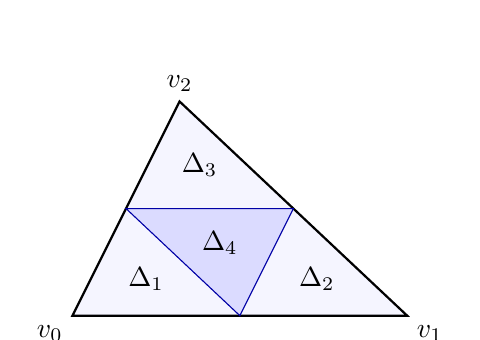
\begin{tikzpicture}[scale=.85]
 \coordinate (a) at (0,0);\coordinate (b) at (5,0);
 \coordinate (c) at (1.6,3.2);\coordinate (ab) at (2.5,0);
 \coordinate (bc) at (3.3,1.6);\coordinate (ca) at (.8,1.6);
 \fill[blue!4] (a)--(b)--(c)--cycle;
 \fill[blue!14] (ab)--(bc)--(ca)--cycle;
 \draw[thick] (a)--(b)--(c)--cycle;
 \draw[blue!65!black] (ab)--(bc)--(ca)--cycle;
 \node at (1.1,.55) {$\Delta_1$};\node at (3.65,.55) {$\Delta_2$};
 \node at (1.9,2.25) {$\Delta_3$};\node at (2.2,1.08) {$\Delta_4$};
 \node[below left] at (a) {$v_0$};\node[below right] at (b) {$v_1$};
 \node[above] at (c) {$v_2$};
\end{tikzpicture}
\caption{Each internal edge occurs twice with opposite orientations.
The proof processes all four children; it does not choose a ``worst''
triangle or construct a nested limiting point.}
\end{figure}

\begin{theorem}[The strictly finite Cauchy estimate]\label{thm:finitec}
If \(D_\Delta2^{-m}\le2^{-\mu(k)}\), then
\begin{equation}\label{eq:finitec}
 \boxed{\quad
 \norm{\trap_{m,n}(f;\bd\Delta)}
 \le D_\Delta P_\Delta2^{-k}
   +P_\Delta2^{-n}\bigl(2^{m+1}+D_\Delta\bigr).
 \quad}
\end{equation}
This is a theorem about finite rational expressions, before any use of
integral notation.
\end{theorem}
\begin{proof}
On one small triangle choose a vertex \(a\) and subtract the rational
complex-affine function
\(A(z)=F(a,n)+D(a,n)(z-a)\).
Put \(d=D_\Delta2^{-m}\), \(p=P_\Delta2^{-m}\).
At every vertex of the small triangle, \eqref{eq:ud} bounds the
remainder by
\(2^{-k}d+2^{-n}(2+d)\).
The boundary trapezoidal sum of \(A\) is zero by
Lemma~\ref{lem:algebra}. The three edge errors therefore total at most
\[
 p\bigl(2^{-k}d+2^{-n}(2+d)\bigr).
\]
Sum this inequality over the \(4^m\) triangles. Every internal edge
cancels exactly; the remaining subdivided outer edges are precisely
\(\trap_{m,n}(f;\bd\Delta)\). Now use
\(4^m pd=P_\Delta D_\Delta\) and
\(4^mp=P_\Delta2^m\). This is \eqref{eq:finitec}.
\end{proof}

The sample-error term grows with \(2^m\), because we bounded errors on
all small triangles before cancellation. It would be incorrect to omit
this factor while keeping the same finite proof. The sample precision
below explicitly absorbs it. The analytic error stays bounded because
\(4^m\) is exactly balanced by two factors \(2^{-m}\).

For a finite triangle chain \(T=\sum_\ell c_\ell\Delta_\ell\), let
\begin{equation}\label{eq:chainbudgets}
 A_T=\sum_\ell|c_\ell|D_\ell P_\ell,\quad
 L_T=\sum_\ell|c_\ell|P_\ell,\quad
 D_* =\max_\ell D_\ell.
\end{equation}
Use conforming edge subdivisions so shared edges have the same endpoint
codes. If extra boundary vertices have been inserted, first triangulate
the affected cells by a rational centre fan; this is a finite operation.
The moduli can be the maxima over the finitely many carriers.
Summing \eqref{eq:finitec} proves
\begin{equation}\label{eq:finitechain}
 \norm{\trap_{m,n}(f;\bd T)}
 \le A_T2^{-k}+2^{-n}\bigl(2^{m+1}L_T+A_T\bigr)
\end{equation}
whenever \(D_*2^{-m}\le2^{-\mu(k)}\).

Here is a complete precision schedule. Put
\begin{align}
 b&=\sigma(1+A_T+L_T+D_*),\notag\\
 k&=q+b+4,\qquad m=\max\{\mu(k),\nu(k)\}+b,\notag\\
 n&=q+m+b+5.\label{eq:cauchyschedule}
\end{align}
The three terms on the right of \eqref{eq:finitechain} are at most
\(2^{-q-4},2^{-q-4},2^{-q-5}\), respectively. Thus
\begin{equation}\label{eq:cauchyoutput}
 \norm{\trap_{m,n}(f;\bd T)}\le\tfrac5{32}2^{-q}<2^{-q}.
\end{equation}
The mesh simultaneously satisfies the continuity requirement. Comparing
this schedule with \eqref{eq:integralname} by a common refinement and
Lemma~\ref{lem:quadrature} proves \(\Int_{\bd T}(f)=0\).
This proves Theorem~\ref{thm:previewc} with its claimed arithmetic meaning.

\begin{corollary}[Convex domains and path independence]\label{cor:convex}
If a rational polygonal closed chain lies in a convex certified carrier,
then its integral is zero. Integrals along two rational polygonal paths
in that carrier with the same endpoints agree.
\end{corollary}
\begin{proof}
Choose a rational base point \(b\) in the carrier. For each oriented edge
\([u,v]\), use the signed triangle \([b,u,v]\). Convexity keeps every
triangle in the carrier. Radial edges cancel by the incidence condition,
so their total boundary is the original chain. For path independence
apply this to the first path minus the second.
\end{proof}

\section{A primitive theorem and all square moments}\label{sec:moments}

\subsection{The primitive theorem is finite telescoping}

Suppose \(H\) has first-order remainder \(f\) along a polygonal path,
with a supplied uniform modulus of the form \eqref{eq:ud}. On any fine
partition, the identity
\[
 H(v_{\rm end})-H(v_{\rm start})
       =\sum_j\bigl(H(x_{j+1})-H(x_j)\bigr)
\]
telescopes. If the remainder per cell is at most
\(\epsilon\norm{x_{j+1}-x_j}\), subtraction of the left-endpoint
quadrature costs at most \(L\epsilon\). At finite evaluation precision
\(n\), for \(N_c\) cells, the direct bound is
\begin{equation}\label{eq:finiteprimitive}
 L\epsilon+(2N_c+L)2^{-n}.
\end{equation}
The endpoint telescoping occurs on the evaluated \(H\)-values themselves.
Choose the mesh by the supplied remainder modulus and the precision by
\eqref{eq:sigma}. Proposition~\ref{prop:rules} identifies left-endpoint
and trapezoidal integrals. We have proved, entirely by finite estimates,
\begin{equation}\label{eq:primitive}
 \Int_{[\text{path}]}(f)=H(v_{\rm end})-H(v_{\rm start}).
\end{equation}

For \(k\ge0\), the primitive of \((z-a)^k\) is
\((z-a)^{k+1}/(k+1)\). A double difference-of-powers identity gives a
quadratic remainder with a rational bound on each bounded carrier.
For \(k=-t-1\), \(t\ge1\), use
\(H(z)=-(z-a)^{-t}/t\). If the endpoint inverse norms are bounded by
\(U\), write \(u=z-a\), \(v=w-a\), \(h=v-u\), and use
\begin{align}
 H(w)-H(z)&=\frac h t
       \sum_{j=0}^{t-1}v^{-j-1}u^{-t+j},\label{eq:negativepower}\\
 \norm{v^{-p}-u^{-p}}&\le pU^{p+1}\norm h.\notag
\end{align}
The first identity becomes the finite positive-power difference identity
after clearing denominators; the second applies that identity to the
inverses. Subtract \(hu^{-t-1}\) from \eqref{eq:negativepower} and sum
\(j+1\) to get remainder bound
\begin{equation}\label{eq:negativeTaylor}
 \frac{t+1}{2}U^{t+2}\norm h^2.
\end{equation}
These formulas give PR moduli uniformly in the integer exponent.
Consequently
\begin{equation}\label{eq:ordinarymoments}
 \Int_\Gamma((z-a)^k)=0\qquad(k\in\Z,\ k\ne-1)
\end{equation}
for every closed polygonal chain with the required inverse separation
when negative exponents occur. We have not invoked a classical
fundamental theorem of calculus.

\subsection{A fast rational construction of \texorpdfstring{\(\pi\)}{pi}}

For \(0\le t\le1\), the finite geometric identity gives
\begin{equation}\label{eq:pigeometric}
 \frac1{1+t^2}
 =\sum_{j=0}^{N-1}\frac{(1-t^2)^j}{2^{j+1}}
   +\frac{((1-t^2)/2)^N}{1+t^2}.
\end{equation}
The remainder is between zero and \(2^{-N}\), uniformly.
Polynomial integration here means the finite linear rule
\(\int_0^1t^n\dd t=1/(n+1)\), justified by the telescoping primitive
proof above. Set
\begin{equation}\label{eq:piapprox}
 J_j=\sum_{\ell=0}^{j}
       \frac{(-1)^\ell\binom j\ell}{2\ell+1},\quad
 p_N=4\sum_{j=0}^{N-1}\frac{J_j}{2^{j+1}}.
\end{equation}
Integration of \eqref{eq:pigeometric} proves
\begin{equation}\label{eq:pibound}
 p_N\le\pi:=4\int_0^1\frac{\dd t}{1+t^2}
          \le p_N+4\,2^{-N},\qquad 2\le\pi\le4.
\end{equation}
The integral is the rational-sum construction of Section~\ref{sec:integral}
on a real segment; its integrand has explicit Lipschitz constant \(2\).
Thus \(p_{n+3}\) gives a PR name of error at most \(2^{-n-1}\).
For efficient evaluation the same finite polynomials satisfy
\begin{equation}\label{eq:Jrec}
 J_0=1,\qquad J_j=\frac{2j}{2j+1}J_{j-1}\quad(j\ge1).
\end{equation}
To prove the recurrence, integrate the derivative of
\(t(1-t^2)^j\): its endpoint difference is zero and it yields
\(J_j=2j(J_{j-1}-J_j)\). This is a polynomial identity under finite
integration, not integration by parts assumed from analysis.

This normalization is the ordinary constant \(\pi\). One direct
identification uses the rational unit-circle parametrization
\(w(t)=(1+it)/(1-it)\), \(0\le t\le1\). It runs from \(1\) to \(i\),
satisfies \(|w(t)|=1\), and its speed is \(2/(1+t^2)\), as follows by
differentiating the rational expression and squaring the norm.
Its four quarter-arcs therefore have total length
\(8\int_0^1(1+t^2)^{-1}\dd t=2\pi\). This explanatory identification
does not enter the finite arithmetic proof.

\subsection{The exceptional square moment}

Let \(Q_r(a)=\{z:|z-a|_\infty\le r\}\), with counterclockwise boundary,
where \(a\in\Q(i)\) and \(r>0\) is rational. Its taxicab perimeter is
\(8r\). On the right side write \(z-a=r(1+it)\), \(-1\le t\le1\).
Then the rational identity
\[
 \frac{\dd z}{z-a}=\frac{t+i}{1+t^2}\dd t
\]
holds. The real part integrates to zero by exact pairing of opposite
sample points. The imaginary part is
\(2i\int_0^1(1+t^2)^{-1}\dd t\).
Multiplication of both \(z-a\) and \(\dd z\) by \(i\) leaves the quotient
unchanged, so the four oriented sides contribute equally. Thus
\begin{equation}\label{eq:kernelmoment}
 \Int_{\bd Q_r(a)}((z-a)^{-1})=2\pi i.
\end{equation}
Together with \eqref{eq:ordinarymoments}, this proves
\begin{equation}\label{eq:allmoments}
 \boxed{\quad
 \Int_{\bd Q_r(a)}((z-a)^k)=
 \begin{cases}2\pi i,&k=-1,\\0,&k\ne-1.\end{cases}
 \quad}
\end{equation}
This proof uses no logarithm, argument function, pre-existing winding
theorem, or residue formula. All changes of parametrization are affine
identities of rational sample lists, followed by
Proposition~\ref{prop:rules}.

\section{An annular Cauchy formula and a derived Laurent expansion}\label{sec:laurent}

Fix \(a\in\Q(i)\), \(r>0\), and
\begin{equation}\label{eq:radii}
 s=r/8,\qquad R=8r.
\end{equation}
Assume the data of Definition~\ref{def:hol} on the closed square annulus
\(K=Q_R(a)\setminus\operatorname{int}Q_s(a)\).
Let \(M_R,M_s\) bound \(\norm f\) on its outer and inner boundaries.
A single bound on \(K\) may be used for both. All integrals in this
section are the already constructed names.

\subsection{The annular formula}

\begin{theorem}[Annular Cauchy formula]\label{thm:annular}
For every rational \(z\in\bd Q_r(a)\),
\begin{equation}\label{eq:annular}
 2\pi i f(z)=
 \Int_{\bd Q_R(a)}\!\left(\frac{f(\zeta)}{\zeta-z}\right)
 -\Int_{\bd Q_s(a)}\!\left(\frac{f(\zeta)}{\zeta-z}\right).
\end{equation}
The equality has PR precision bounds uniform in these \(z\).
\end{theorem}
\begin{proof}
For an arbitrary accuracy index \(k\), choose the positive rational
\begin{equation}\label{eq:smallh}
 h=\min\bigl\{(r-s)/4,\ (R-r)/4,\ 2^{-\nu(k)-1}\bigr\}.
\end{equation}
Then \(Q_h(z)\) is disjoint from \(Q_s(a)\) and inside
\(\operatorname{int}Q_R(a)\). Every point of its boundary is within
taxicab distance \(2h\le2^{-\nu(k)}\) of \(z\).

Draw all vertical and horizontal lines through the sides of these three
squares. There are at most six coordinates on either axis, so at most
25 grid rectangles. Keep the rectangles inside the outer square and
outside both inner square interiors, and split each into two triangles.
Boundary cancellation is literally
\[
 \bd T_h=\bd Q_R(a)-\bd Q_s(a)-\bd Q_h(z),
\]
with edges split at the grid vertices. The carrier avoids \(z\) by
\(|\zeta-z|_\infty\ge h\). Thus the quotient in
\eqref{eq:annular} has the explicit PR data supplied by
\eqref{eq:quotientremainder}, with \(A=2/h\).
Apply Cauchy's theorem to these at most 50 triangles. It gives
\begin{equation}\label{eq:annularhole}
 \Int_{\bd Q_R(a)}\!\left(\frac{f(\zeta)}{\zeta-z}\right)
 -\Int_{\bd Q_s(a)}\!\left(\frac{f(\zeta)}{\zeta-z}\right)
 =\Int_{\bd Q_h(z)}\!\left(\frac{f(\zeta)}{\zeta-z}\right).
\end{equation}
On the last boundary, replacing \(f(\zeta)\) by \(f(z)\) changes the
integral by at most
\begin{equation}\label{eq:smallerror}
 (8h)(2/h)2^{-k}=16\,2^{-k}.
\end{equation}
The constant part equals \(2\pi i f(z)\) by
\eqref{eq:kernelmoment}. Given a final precision \(q\), take
\(k\ge q+5\) and carry out the finite Cauchy stage at the additional
precision prescribed by \eqref{eq:cauchyschedule}; all its bounds are
PR in \(h\). Evaluate the finite names with the remaining error budget.
The discrepancy in \eqref{eq:annular} is then arbitrarily small.
Lemma~\ref{lem:closure} gives the equality. There is no search for a
neighbourhood and no interchange of two unspecified limits.
\end{proof}

\subsection{Coefficients and a quantitative tail}

Define coefficients, for \(n\ge0\), by
\begin{align}
 a_n&=(2\pi i)^{-1}
      \Int_{\bd Q_R(a)}\bigl(f(\zeta)(\zeta-a)^{-n-1}\bigr),
       \label{eq:poscoeff}\\
 a_{-n-1}&=(2\pi i)^{-1}
      \Int_{\bd Q_s(a)}\bigl(f(\zeta)(\zeta-a)^n\bigr).
       \label{eq:negcoeff}
\end{align}
The reciprocal of \(2\pi i\) is available with a PR modulus because
\(\pi\ge2\). The integral construction and the kernel closure estimates
make these coefficients PR names, uniformly in the signed index and
requested accuracy, for each fixed input presentation.

\begin{theorem}[Derived Laurent approximation]\label{thm:laurent}
For \(z\in\bd Q_r(a)\) and every integer \(N\ge1\),
\begin{equation}\label{eq:laurenttail}
 \boxed{\quad
 \norm{f(z)-\sum_{k=-N}^{N-1}a_k(z-a)^k}
 \le C_r2^{-N},\qquad
 C_r=\frac{16RM_R}{R-r}+\frac{16sM_s}{r-s}.
 \quad}
\end{equation}
In particular \(C_r\le20(M_R+M_s)\). The same calculation proves
the representation throughout the open band
\(r/2<|z-a|_\infty<2r\), with suitable explicit ratios strictly below
one and uniform rates on smaller closed subbands.
\end{theorem}
\begin{proof}
Write \(u=\zeta-a\), \(v=z-a\). On the outer square,
\(\norm v\le2r\), \(\norm{u^{-1}}\le2/R\), so
\(\norm{v/u}\le1/2\). On the inner square,
\(\norm u\le2s\), \(\norm{v^{-1}}\le2/r\), so
\(\norm{u/v}\le1/2\). Use only the finite identities
\begin{align}
 \frac1{u-v}
   &=\sum_{n=0}^{N-1}\frac{v^n}{u^{n+1}}
          +\frac{(v/u)^N}{u-v},\label{eq:geomouter}\\
 \frac1{u-v}
   &=-\sum_{n=0}^{N-1}\frac{u^n}{v^{n+1}}
          +\frac{(u/v)^N}{u-v}.\label{eq:geominner}
\end{align}
They follow by multiplying the finite geometric-sum identity by the
nonzero denominators. There is no infinite series interchange.

In \eqref{eq:annular}, substitute \eqref{eq:geomouter} for the outer
integral and \eqref{eq:geominner} for the inner integral. Finite
linearity yields exactly the sum in \eqref{eq:laurenttail}, with the
coefficients \eqref{eq:poscoeff}--\eqref{eq:negcoeff}.
On the outer contour \(|u-v|_\infty\ge R-r\), so its remainder integral
has norm at most
\[
 (8R)M_R\frac{2}{R-r}\,2^{-N}.
\]
The inner remainder is bounded by
\((8s)M_s\,2(r-s)^{-1}2^{-N}\).
Finally \(\norm{(2\pi i)^{-1}}=1/(2\pi)\le1\), giving
\eqref{eq:laurenttail}. The displayed simpler constant follows by
substituting \(R=8r,s=r/8\).

For the open band, put \(t=|v|_\infty\). The two sufficient norm ratios
are \(4t/R=t/(2r)<1\) and \(4s/t=r/(2t)<1\).
The small-square argument remains valid, and the same finite identities
give geometric convergence. Rational subband margins bound both ratios
away from one and give PR rates as in Section~\ref{sec:data}.
\end{proof}

To reach uniform error \(2^{-q}\) on the middle square it suffices to
take \(N\ge q+\sigma(C_r)\), with \(N\ge1\). If the finite sum is itself
numerically evaluated, coefficient errors also have an explicit budget.
Put \(U=\max(1,2r,2/r)\); then
\(\norm{(z-a)^k}\le U^{|k|}\). Approximating each coefficient to error
\(\eta\) costs at most
\(\eta\sum_{k=-N}^{N-1}U^{|k|}\). A bounded \(\sigma\)-shift makes this
as small as required. Thus the assertion is a literal approximation
algorithm, not just a formal Laurent series.

\subsection{Independence, uniqueness, and essential singularities}

For any signed integer \(m\), the function
\(f(\zeta)(\zeta-a)^{-m-1}\) has effective holomorphy data on a closed
annulus avoiding \(a\). The finite rectangular-grid filling and Cauchy's
theorem show that its integrals over two concentric square boundaries
are equal. This proves radius independence of the coefficient formulas
whenever the intervening annulus is part of the supplied domain.

To verify directly that the constructed coefficient is the unique one,
fix \(m\) and take \(N>|m|\). Multiply the tail estimate by
\((z-a)^{-m-1}\) on \(\bd Q_r(a)\) and integrate. By
\eqref{eq:allmoments}, only the term with index \(m\) survives:
\[
 \norm{\Int_{\bd Q_r(a)}
       \bigl(f(z)(z-a)^{-m-1}\bigr)-2\pi i a_m}
 \le8r\,U^{|m+1|}C_r2^{-N}.
\]
The right side has an explicit PR rate. Therefore
\begin{equation}\label{eq:coefficientunique}
 a_m=(2\pi i)^{-1}\Int_{\bd Q_r(a)}
                         \bigl(f(z)(z-a)^{-m-1}\bigr).
\end{equation}
Any other coefficient sequence given by PR names whose two-sided
truncations converge uniformly on that square with a supplied PR
modulus satisfies the same formula, by the same finite argument, and
hence agrees coefficient by coefficient.

Define \(\Res(f,a)=a_{-1}\). This coefficient is independently derived
and characterized by the Laurent approximation. Although
\eqref{eq:coefficientunique} also gives an integral formula for it,
we did not merely choose a residue definition to make the global
residue formula automatic. Neither the construction nor the proof
requires that the negative coefficients eventually vanish. Thus they
apply to effectively presented isolated essential singularities.

\section{The residue theorem and an explicit final error budget}\label{sec:residue}

\begin{lemma}[Local residue formula]\label{lem:localres}
Under the preceding annular hypotheses,
\begin{equation}\label{eq:localres}
 \Int_{\bd Q_r(a)}(f)=2\pi i\Res(f,a).
\end{equation}
More explicitly, replacing \(f\) by its \(2N\)-term Laurent polynomial
in this integral costs at most \(8rC_r2^{-N}\).
\end{lemma}
\begin{proof}
Integrate \eqref{eq:laurenttail} and use
\eqref{eq:integralbound}. Every term except \(a_{-1}(z-a)^{-1}\)
has zero moment; that term has moment \(2\pi i a_{-1}\).
Choose \(N\) with \eqref{eq:sigma} for each requested accuracy.
\end{proof}

Now take the input of Theorem~\ref{thm:previewr}. Cauchy's theorem on
each triangle of \(T\), with its integer multiplicity, and
\eqref{eq:certificate} give
\[
 \Int_\Gamma(f)=\sum_jw_j\Int_{\bd Q_{r_j}(a_j)}(f).
\]
Substitute Lemma~\ref{lem:localres}. This proves
\begin{equation}\label{eq:globalres}
 \boxed{\quad
 \Int_\Gamma(f)=2\pi i\sum_jw_j\Res(f,a_j).
 \quad}
\end{equation}
All sums are finite, including the sum over singularities.

\subsection{An arithmetical output statement}

Here is a useful concrete form of the conclusion. Let \(q_\Gamma\) be a
rational approximation of the contour integral with error
\(\eta_\Gamma\), let \(q_j\) approximate the residue at \(a_j\) with
error \(\eta_c\), and let \(q_\pi\) approximate \(\pi\) with error
\(\eta_\pi\), where \(|q_\pi|\le5\). Take known bounds
\(b_j\ge\norm{\Res(f,a_j)}\) and put
\[
 W=\sum_j|w_j|,\qquad B_*=\sum_j|w_j|b_j.
\]
The coefficient formula permits, for example,
\(b_j=8s_jM_{s_j}\), since \(\norm{(2\pi i)^{-1}}\le1\).
Finite product and sum estimates give
\begin{equation}\label{eq:outputerror}
 \norm{q_\Gamma-2q_\pi i\sum_jw_jq_j}
 \le\eta_\Gamma+2B_*\eta_\pi+10W\eta_c.
\end{equation}
Choosing
\begin{align*}
 \eta_\Gamma&\le2^{-q-2},\\
 \eta_\pi&\le2^{-q-2-\sigma(1+2B_*)},\\
 \eta_c&\le2^{-q-2-\sigma(1+10W)}
\end{align*}
makes the right side at most \(3\cdot2^{-q-2}<2^{-q}\).
The integral algorithm, \eqref{eq:piapprox}, and the coefficient
algorithms supply exactly these rational approximations.

To expand the proof into one finite verification at precision \(q\),
retain instead a Cauchy residual \(E_T\) from
\eqref{eq:finitechain}, and local truncation residuals. The bound is
\begin{equation}\label{eq:expandedbudget}
 E_T+\sum_j|w_j|8r_jC_j2^{-N_j}
       +\eta_\Gamma+2B_*\eta_\pi+10W\eta_c,
\end{equation}
with any auxiliary quadrature and finite-coefficient evaluation errors
allocated to the corresponding three \(\eta\)-budgets.
For example take \(E_T\le2^{-q-4}\),
\(N_j\ge q+4+\sigma(1+\sum_j|w_j|8r_jC_j)\), and each of the last
three terms at most \(2^{-q-4}\). The combined bound is then less than
\(2^{-q}\). The Cauchy schedule is explicit even when local hole radii
depend on \(q\); all resulting meshes and sample precisions remain PR.
This describes the arithmetic conclusion without relying on a
qualitative assertion that some error will eventually be small.

\section{Finite planar fillings and winding numbers}\label{sec:geometry}

This section supplies the geometric content of
\eqref{eq:certificate}. It also makes clear which domain hypothesis is
needed in a multiply connected region.

\subsection{Rectangles and square holes}

If a closed rational rectangle contains finitely many pairwise disjoint
closed rational rectangular holes strictly in its interior, draw the
vertical and horizontal lines through every outer and hole side.
For each resulting elementary rectangle, use its rational midpoint to
decide whether it lies outside all hole interiors. Keep exactly those
rectangles, each split into two consistently oriented triangles.
No elementary rectangle crosses a hole side. Shared edges cancel, so
\begin{equation}\label{eq:gridboundary}
 \bd T=\bd R_{\rm outer}-\sum_j\bd R_j.
\end{equation}
This is the complete geometric proof used for the annular Cauchy formula.
For a single annulus, it also proves radius independence of integrals.

\subsection{A general rational polygonal cycle}

\begin{theorem}[Finite planar filling]\label{thm:filling}
Let \(\Gamma\) be a closed rational polygonal integer chain and let
\(Q_1,\ldots,Q_J\) be pairwise disjoint rational closed squares,
disjoint from the carrier of \(\Gamma\). There is an explicit PR
construction of integers \(w_j\) and a rational triangle chain \(T\)
outside the square interiors such that
\[
 \bd T=\Gamma-\sum_jw_j\bd Q_j.
\]
The statement is a plane-geometric construction. It does not assert that
this particular filling lies inside an arbitrarily prescribed open set.
\end{theorem}
\begin{proof}
We describe the construction and verify every type of edge coefficient.
Zero-length edges may first be deleted.

\emph{Arrangement.} Form the segment arrangement of \(\Gamma\) and all
square boundaries. Two nonparallel segments intersect by solving a
two-by-two rational system and checking rational parameter intervals.
For parallel segments test collinearity; overlapping ones are split at
all their endpoints. Include every intersection and endpoint in a
common vertex list, split each segment at all its incident vertices,
and add integer multiplicities of coincident pieces. With \(E\) original
segments, an initial vertex bound is \(V\le2E+E^2\).
All sorting and incidence operations are bounded finite loops.

\emph{Generic height.} Choose an integer \(t\) so the shear
\((x,y)\mapsto(x,y+tx)\) gives distinct heights to distinct vertices.
A pair forbids at most one integer value of \(t\); if its \(x\)-coordinates
agree and the vertices are distinct, it forbids none. Search
\(0,\ldots,V(V-1)/2\). There are one more candidates than possible
forbidden values, so a candidate succeeds. This finite counting fact
can be checked by assigning to each failed candidate its first forbidden
pair; a pair cannot be assigned twice. Thus no nondegenerate arrangement
edge is horizontal. The shear has determinant one. It is used only for
the rational triangulation; transform vertices back before applying any
analytic estimate.

\emph{Strip cells.} Add a rational rectangle strictly enclosing the
sheared arrangement. Include its top and bottom heights in the strip
list, and at every arrangement-vertex height draw a horizontal segment
across it. Within an open strip between successive
heights, every active edge is the graph of a rational affine function
of height. No two such graphs cross in the strip, since all intersections
are already vertices. Sort their order using the rational middle
height. The cells between successive graphs are convex rational
trapezoids or triangles. Boundary coordinates are obtained by rational
line intersection.

\emph{Labels.} For a cell choose a rational interior point and put
\begin{equation}\label{eq:raylabel}
 w=\sum_{\substack{e\text{ a piece of }\Gamma\\
                  e\text{ to the right of the point}}}
       m(e)\operatorname{sgn}(y_{
m end}(e)-y_{
m start}(e)).
\end{equation}
Only edges crossing the cell's strip participate. This is a finite
right-ray crossing count. The rightmost cell has label zero.
Crossing an upward oriented edge from right to left adds its
multiplicity; crossing a downward oriented edge subtracts it.
Accordingly the label on the left of any oriented \(\Gamma\) edge
minus that on its right is exactly its multiplicity. Square edges alone
do not change the label.

\emph{Horizontal seams.} Compare labels just below and above a vertex
height, at a seam point other than a vertex. Edges not incident with the
unique vertex at that height have matching contributions. If the vertex
is to the left of the ray, incident edges contribute nothing. If it is
to the right, the change in their signed contribution is the total
outgoing multiplicity minus the incoming multiplicity at the vertex.
This is zero because \(\bd\Gamma=0\). Splitting an original edge at an
intersection adds equal incoming and outgoing multiplicities, so the
condition persists at new vertices. Thus the two cell labels agree
across every artificial horizontal seam.

\emph{Exterior and hole labels.} The label also vanishes in the far
left exterior. For a generic horizontal line, the total signed crossing
number of the closed chain is zero: sum the zero vertex divergences
over vertices above the line; only crossing edges remain, with exactly
these signs. All exterior boundary coefficients are therefore zero.
Inside each square, labels are constant. To see this finitely, connect
interior rational cell points by a segment in the convex square,
perturbed through a rational intermediate point to avoid the finitely
many arrangement vertices and lines of coincidence. Such a point can
be selected by bounded search: place more candidate points on a small
rational line segment than there are forbidden intersections, choosing
the segment direction by the same finite avoidance argument as for the
shear. Along the resulting finite path every crossed subdivision edge
has zero label difference, because no \(\Gamma\) edge meets the square.
Call the common label \(w_j\).

\emph{Triangles and cancellation.} First split every horizontal cell
side at all endpoints induced by either adjacent strip. For each
nondegenerate convex cell take its rational vertex average, an interior
point, and fan to the resulting cyclic boundary list. This makes
horizontal subdivisions match literally. Give each triangle outside
the square interiors its cell label as multiplicity, and discard the
triangles inside the squares. Internal fan edges cancel. Across an
arrangement edge the remaining coefficient is the left label minus
the right label; it is the required \(\Gamma\) multiplicity. Across
horizontal seams it is zero. Along a counterclockwise square boundary
the removed inside is on the left, so the remaining coefficient is
\(-w_j\). The artificial outer rectangle contributes zero. These are
all the edges, proving the claimed boundary identity.

For an explicit finite bound, pad all lists to
\(100(E+V+10)^6\) entries. There are at most \(E(V+1)\) initial atomic
edges, at most \(V+1\) strips, and at most that many further horizontal
cuts per atomic edge. Taking all pairs again for seam incidence and
cell boundaries is still below this generous polynomial bound.
Each triangle fan has no more pieces than its finite subdivided boundary
list. Rational arithmetic and the bounded searches above are PR, so
the entire construction is PR. No unspecified triangulation theorem is
being used.
\end{proof}

For application in an open set \(U\), either provide a different
filling whose cells have certified analytic data in \(U\), or verify
that every nonzero-label triangle of this construction has those data.
This is precisely the effective content replacing the usual
null-homology-in-\(U\) condition. Local holomorphy near \(\Gamma\) alone
does not imply it; for example \(1/z\) is holomorphic near a square
surrounding zero but has nonzero square integral.

\subsection{The indices are intrinsic winding numbers}

\begin{proposition}\label{prop:winding}
For a certificate \eqref{eq:certificate} avoiding all centres,
\begin{equation}\label{eq:winding}
 (2\pi i)^{-1}\Int_\Gamma((z-a_j)^{-1})=w_j.
\end{equation}
Consequently any two such certificates yield the same integers.
\end{proposition}
\begin{proof}
Apply Cauchy's theorem on \(T\) to \(1/(z-a_j)\), using its supplied
positive separation. Its integral on \(Q_{r_j}(a_j)\) is \(2\pi i\).
For \(\ell\ne j\), the kernel is holomorphic on the entire square
\(Q_{r_\ell}(a_\ell)\), since the squares are disjoint. A two-triangle
filling and Cauchy's theorem show that this other integral is zero.
The chain identity gives \eqref{eq:winding}. If two integer indices
differ, their difference has absolute value at least one, whereas
\(\pi\ge2\) and the corresponding named integral difference is zero.
That is a contradiction at an explicitly chosen accuracy, so the
integers agree. Only decidable integer comparison is involved.
\end{proof}

Equation~\eqref{eq:raylabel} therefore computes these winding numbers
using rational comparisons, and \eqref{eq:winding} identifies them with
the usual analytic normalization. For a positively oriented rectangular
outer contour containing all the squares, the grid filling gives
\(w_j=1\). More complicated, multiply traversed, negatively oriented,
or self-intersecting polygonal cycles are handled by the same signed
integer formula. No classification of Jordan curves is required.

\section{Effective rectifiable curves and uniform homotopies}\label{sec:curves}

The preceding polygonal theorems extend to curves with supplied
quantitative data. This extension is proved here, rather than left as
an unspecified approximation argument. The singularity centres in the
residue corollary remain rational. No claim is made that a merely
computable curve automatically comes with the bounds below.

\subsection{Curve data and finite Stieltjes sums}

Let \(G(t,p)\in\Q(i)\) be a fixed PR name for \(\gamma(t)\), for rational
\(t\in[0,1]\). Give a nondecreasing PR continuity modulus \(\nu_\gamma\)
and a rational variation bound \(L\) such that
\begin{align}
 |s-t|\le2^{-\nu_\gamma(a)}&\ \Longrightarrow\
       \norm{\gamma(s)-\gamma(t)}\le2^{-a},\label{eq:curvemod}\\
 \sum_{j<2^m}\norm{\gamma((j+1)/2^m)-\gamma(j/2^m)}
       &\le L\qquad\text{for every }m.\label{eq:curvevar}
\end{align}
Assume \(\gamma(0)=\gamma(1)\). These are arithmetical statements about
names. For example the rational version of \eqref{eq:curvevar} has
\(G(\cdot,p)\) in place of \(\gamma\) and right side
\(L+2^{m+1-p}\); requiring it for all \(m,p\) gives exactly the stated
bound. The usual total variation bound implies \eqref{eq:curvevar}.
Only these dyadic instances are needed for the definition below.

Give a positive rational collar width \(\rho\). The \(f\)-data, including
bound \(M\) and modulus \(\nu_f\), are valid on the \(\rho\)-collar of
the curve. For Cauchy conclusions the first-order differentiability
data are valid there too. This does not require a new set variable:
one may state the uniform rational contracts on balls around rational
curve samples, reducing their radii by the known approximation error.
Every constructed triangle is then certified to lie in one such ball.
Composition \(f(\gamma(t))\) has a PR name: approximate \(\gamma(t)\)
at the precision required by \(\nu_f(a+1)\) and the collar margin, then
evaluate \(f\) to accuracy \(2^{-a-1}\).

Consider the finite expressions in names
\[
 S_m=\sum_{j<2^m}f(\gamma(j/2^m))
                 \bigl(\gamma((j+1)/2^m)-\gamma(j/2^m)\bigr).
\]
If \(n\ge m\ge\nu_\gamma(\nu_f(r))\), group fine increments by their
coarse interval and telescope them. This gives the exact identity
\[
 S_n-S_m=\sum_{\text{coarse }j}\sum_{\text{fine }\ell\text{ in }j}
 [f(\gamma(\ell/2^n))-f(\gamma(j/2^m))]
 [\gamma((\ell+1)/2^n)-\gamma(\ell/2^n)].
\]
The two moduli bound the first bracket by \(2^{-r}\), and
\eqref{eq:curvevar} bounds the sum of the second norms by \(L\).
Consequently
\begin{equation}\label{eq:stieltjesrefine}
 \norm{S_n-S_m}\le L2^{-r}.
\end{equation}
It remains to make these sums completely rational, with controlled node
errors; finite sums of abstract names alone are not yet the algorithm.

\subsection{Rationalization and an explicit integral name}

Put \(N=2^m\). Choose rational nodes \(q_j\) with
\(\norm{q_j-\gamma(j/N)}\le\eta\), and force \(q_N=q_0\).
Closedness preserves this error bound at the last endpoint. Let
\(V(q)=\sum_{j<N}\norm{q_{j+1}-q_j}\) and
\(T(q)=\sum_{j<N}f(q_j)(q_{j+1}-q_j)\).
If \(\eta\le2^{-\nu_f(r)}\) and nodes are in the collar, then
\begin{align}
 V(q)&\le L+2N\eta,\label{eq:nodevar}\\
 \norm{T(q)-S_m}&\le L2^{-r}+2MN\eta.\label{eq:nodeerror}
\end{align}
For the proof put \(e_j=q_j-\gamma(j/N)\). Subtract the sums and use
\[
 T(q)-S_m=\sum_j[f(q_j)-f(\gamma(j/N))]\Delta\gamma_j
              +\sum_j f(q_j)(e_{j+1}-e_j).
\]
The two terms give \eqref{eq:nodeerror}; the same increment identity
gives \eqref{eq:nodevar}. Replacing \(f(q_j)\) by an approximation
\(v_j\) of error \(\zeta\) adds at most \(\zeta(L+2N\eta)\).

Choose \(b,C\in\N\) with
\(\max(1,L,M)\le2^b\) and \(2^{-C}\le\rho/8\), using bounded rational
search. For precision \(k\) set
\begin{align}
 r&=k+b+4, &h&=\max\{\nu_f(r)+2,C\},\notag\\
 m&=\max\{k,\nu_\gamma(h)\}, &
 p&=\max\{h,m+k+b+3\},\notag\\
 q_j&=G(j/2^m,p)\quad(j<2^m), &q_{2^m}&=q_0,\notag\\
 A_\gamma(k)&=\sum_{j<2^m}F(q_j,r)(q_{j+1}-q_j).
       \label{eq:curvealgorithm}
\end{align}
Here \(\eta=2^{-p}\), \(\zeta=2^{-r}\). The schedule gives
\(2N\eta\le1\), \(2MN\eta\le2^{-k-2}\), and
\((3L+1)2^{-r}\le2^{-k-2}\).
Comparing any two \(A_\gamma\)-values through a common dyadic refinement
of the corresponding \(S_m\), using \eqref{eq:stieltjesrefine} and
\eqref{eq:nodeerror}, proves
\[
 \norm{A_\gamma(k)-A_\gamma(\ell)}
       \le2^{-k-1}+2^{-\ell-1}.
\]
Thus \(A_\gamma\) is a regular PR name. Define
\(\Int_\gamma(f)\) to be this name. Under the usual complex
interpretation it is the contour Riemann--Stieltjes integral. Comparing
tagged sums with left-endpoint sums uses the same composed modulus and
variation estimate. For arbitrary rational partitions one supplies the
usual variation bound on those partitions; it follows for continuous
curves from the dyadic bound by approximating the finitely many partition
points with the given modulus. No completion principle is needed for
the arithmetic definition.

\begin{lemma}[Controlled polygon approximation]\label{lem:polygonapprox}
Let \(P_k\) join the nodes in \eqref{eq:curvealgorithm} by straight
segments. Then
\begin{equation}\label{eq:polygonerror}
 \norm{\Int_{P_k}(f)-\Int_\gamma(f)}
 \le(3L+1)2^{-r}+2MN\eta\le2^{-k-1}.
\end{equation}
The assertion remains valid if \(m,p\) are increased above their
displayed lower bounds.
\end{lemma}
\begin{proof}
Every polygon edge has length at most \(3\,2^{-h}\le2^{-\nu_f(r)}\).
Its points lie within \(4\,2^{-h}\le\rho/2\) of the corresponding exact
curve node, so are in the certified collar. Replacing the integrand along
each edge by its left endpoint value costs at most
\((L+1)2^{-r}\), by \eqref{eq:nodevar}. Equation~\eqref{eq:nodeerror}
costs \(L2^{-r}+2MN\eta\), and \eqref{eq:stieltjesrefine} compares
\(S_m\) with the integral name at cost \(L2^{-r}\). Add these three
bounds. All uses of name inequalities can be expanded at finite
precisions, as in Lemma~\ref{lem:closure}.
\end{proof}

\subsection{Homotopy invariance from a rational grid}

Let \(H(s,t)\) be a fixed PR name on rational points of \([0,1]^2\),
with a nondecreasing uniform modulus \(\nu_H\) for the taxicab parameter
metric. Require \(H(s,0)=H(s,1)\). Its endpoint curves
\(\gamma_0=H(0,\cdot)\), \(\gamma_1=H(1,\cdot)\) have supplied variation
bounds. The effective holomorphy data hold on a supplied
\(\rho\)-collar of the whole homotopy image.
No rectifiability or differentiability is required of the intermediate
curves \(H(s,\cdot)\).

Choose \(C\) with \(2^{-C}\le\rho/8\), and choose
\(m\ge\nu_H(C)+1\), \(p\ge C\). Approximate each
\(H(i/2^m,j/2^m)\) by \(q_{ij}\in\Q(i)\) to accuracy \(2^{-p}\),
forcing \(q_{i,2^m}=q_{i,0}\). In each parameter-grid cell use the two
image triangles
\[
 [q_{ij},q_{i,j+1},q_{i+1,j+1}],\qquad
 [q_{ij},q_{i+1,j+1},q_{i+1,j}].
\]
There are exactly \(2\cdot4^m\) triangles. The parameter distance
between two cell corners is at most \(2^{1-m}\), so every image vertex
is within \(2\,2^{-C}\le\rho/4\) of the exact lower-left image value.
Convexity of the taxicab ball puts both triangles in the analytic
collar, even when they overlap, reverse orientation, or degenerate.
Their boundaries cancel to \(P_0-P_1\), the difference of the endpoint
polygons. Diagonals cancel inside cells, shared edges between cells,
and the vertical boundary chains because the rows close.

\begin{theorem}[Effective homotopy invariance]\label{thm:homotopy}
Under these data,
\(\Int_{\gamma_0}(f)=\Int_{\gamma_1}(f)\).
In particular a curve with a supplied such nullhomotopy has zero
integral.
\end{theorem}
\begin{proof}
Choose a common \(b\) for both variation bounds and \(M\). For an
arbitrary \(k\), take \(r=k+b+4\),
\(h=\max(\nu_f(r)+2,C)\),
\(m=\max(k,\nu_H(h)+1)\), and
\(p=\max(h,m+k+b+3)\).
The endpoint curves inherit \(\nu_H\), so
Lemma~\ref{lem:polygonapprox} bounds each endpoint approximation error
by \(2^{-k-1}\). Cauchy's finite triangle theorem on the grid gives
\(\Int_{P_0}(f)=\Int_{P_1}(f)\). The two curve integrals differ by at
most \(2^{-k}\). Universally generalizing over \(k\) proves equality.
For a constant endpoint choose all its polygon nodes to be the same
rational approximation; its integral is identically zero.
\end{proof}

This proves the usual simply connected conclusion whenever the term
``simply connected'' is supplied in the effective sense needed here:
for the particular input curve there is a PR uniformly continuous
nullhomotopy with a positive analytic collar. No procedure extracting
that witness from a bare topological proposition is asserted.

\subsection{Residues for effective curves}

One sufficiently close rational polygon actually has the same integral
as the curve. To see this, choose \(C\) with \(2^{-C}\le\rho/8\),
\(m\ge\nu_\gamma(C)\), and node precision \(p\ge C\).
The polygon \(P\), parametrized on the same dyadic grid, satisfies
\(\norm{P(t)-\gamma(t)}\le2\,2^{-C}\le\rho/4\).
The straight homotopy
\[
 H(s,t)=(1-s)\gamma(t)+sP(t)
\]
has its \(\rho/2\)-collar inside the original analytic collar.
Its modulus is explicit. Compute
\(K_P=2^m\max_j\norm{q_{j+1}-q_j}\), and choose
\(d\) with \(\max(1,K_P,\rho/4)\le2^d\).
Then
\[
 \nu_H(a)=\max\{\nu_\gamma(a+2),a+2+d\}
\]
suffices, by changing \(t\) and \(s\) separately in the displayed
homotopy formula. The polygon has a finite computable variation bound.
Theorem~\ref{thm:homotopy} now proves the exact equality
\(\Int_\gamma(f)=\Int_P(f)\).

If \(P\) has the filling certificate and local data of the polygonal
residue theorem, apply that theorem to obtain
\[
 \Int_\gamma(f)=2\pi i\sum_jw_j\Res(f,a_j).
\]
The same homotopy argument for \(1/(z-a_j)\), with a supplied positive
distance from each centre, identifies \(w_j\) with the winding number
of \(\gamma\). This proves a substantive rectifiable-curve version;
the global filling-domain condition is still required.

Finally, effectively presented piecewise \(C^1\) curves fit these
hypotheses when a finite parameter partition, derivative names, uniform
remainder moduli, and speed bounds \(B_j\) are supplied. On each piece,
finite telescoping over a sufficiently fine partition gives
\(\norm{\gamma(v)-\gamma(u)}\le(B_j+\epsilon)(v-u)\).
At arbitrary dyadic \(\epsilon\), rational closure removes the error.
Refining a finite partition by the piece boundaries and summing yields
\(L=\sum_jB_j(t_{j+1}-t_j)\). This derives the required variation bound
without importing a mean value theorem.

\section{Concrete instances and exact-arithmetic validation}\label{sec:examples}

\subsection{Two simple poles}

Take
\[
 f(z)=\frac1z+\frac2{z-1}
\]
and let \(\Gamma\) be the counterclockwise boundary of
\([-2,3]\times[-2,2]\). Its residues are \(1\) at zero and \(2\) at one.
For example, near zero the second summand has the geometric expansion
\(-2\sum_{n\ge0}z^n\), with its elementary explicit tail; near one,
\(1/z=\sum_{n\ge0}(-1)^n(z-1)^n\). These finite geometric identities
and uniqueness of the Laurent coefficients prove the residue claims.
The residue theorem yields
\begin{equation}\label{eq:example}
 \Int_\Gamma\left(\frac1z+\frac2{z-1}\right)=6\pi i.
\end{equation}

The reference program removes squares of half-side \(1/4\) about zero
and one and constructs 26 rational triangles. It checks the exact
signed boundary equation \(\bd T=\Gamma-\bd Q_0-\bd Q_1\).
To apply the derived Laurent theorem with its specific scale separation,
use smaller middle squares of half-side \(1/64\) and outer half-side
\(1/8\). Their outer squares are disjoint. Cauchy on the explicit square
annuli between half-sides \(1/64\) and \(1/4\) identifies the small-square
integrals with the larger numerical hole integrals. Thus the choice of
larger display holes hides no violation of the local annular hypotheses.

On the entire punctured 26-triangle carrier,
\(|z|_\infty,|z-1|_\infty\ge1/4\), so both inverse norm bounds may be
taken as \(8\). Equations~\eqref{eq:inverseTaylor} and
\eqref{eq:inversebound} give a Lipschitz constant \(192\) and
first-order remainder coefficient \(1536\). Thus
\(\nu(k)=k+8\), \(\mu(k)=k+11\) are valid concrete moduli.
One may take \(M=24\), \(B=192\), before the explicit name slacks.
This is a literal instance of the effective hypotheses.

For efficient numerical validation of reciprocal sums, use the exact
interpolation identity
\begin{equation}\label{eq:interpolationinverse}
 \frac{1-t}{u}+\frac t v-\frac1{(1-t)u+tv}
 =\frac{t(1-t)(v-u)^2}{uv((1-t)u+tv)}.
\end{equation}
If all inverse factors are bounded by \(U\), its norm is bounded by
\(U^3t(1-t)\norm{v-u}^2\).
For a sum \(\sum_jc_j/(z-a_j)\), put
\(K=2\sum_j\norm{c_j}U_j^3\). The finite trapezoidal average of
\(t(1-t)\) over \(N\) equal intervals is
\((N^2-1)/(6N^2)\le1/6\). Comparing with every finer sum proves the
certified quadrature error
\begin{equation}\label{eq:numericerror}
 \norm{\trap_{m,n}-\Int}
 \le\frac{K}{12\,4^m}\sum_e\norm{v_e-u_e}^{3}+L2^{-n}.
\end{equation}
This sharper bound is used only for this reciprocal-sum family; the
general Cauchy proof uses \eqref{eq:finitechain}.

At subdivision depth nine and 32-bit dyadic evaluation, the recorded
exact-rational run gives the following decimal displays. The real
components are exactly zero in the stored rational sums.
\begin{center}
\begin{tabular}{lrr}
\toprule
Contour & Imaginary component & Certified error bound\\\midrule
Outer rectangle & \(18.849555246653495\) & \(8.369\cdot10^{-5}\)\\
Square about zero & \(6.283180680792384\) & \(1.749\cdot10^{-4}\)\\
Square about one & \(12.566360671766915\) & \(3.316\cdot10^{-4}\)\\
\bottomrule
\end{tabular}
\end{center}
The program stores exact fractions and an exact rational interval for
\(\pi\); the printed error bounds above are rounded upward. Seven
validation tests cover affine cancellation, subdivision, the finite
Cauchy bound, grid incidence, \(\pi\), the reciprocal interpolation
identity, and the residue example. These checks test the implementation.
They are not proofs of the universal theorems or of iPRA derivability.

\subsection{An essential singularity}

The example \(f(z)=\exp(1/z)\) has residue one. This can be checked
constructively without classifying singularities: on any square avoiding
zero, take \(U\ge\norm{z^{-1}}\) and use
\[
 \exp(1/z)=\sum_{n\ge0}\frac{z^{-n}}{n!}.
\]
For \(N_0\ge\max(1,\lceil2U\rceil)\), successive terms of the
absolute tail have ratio at most \(1/2\). Therefore the tail after
\(N=N_0+d\) is bounded by
\(2U^{N_0}/N_0!\cdot2^{-d}\). This is an explicit PR rate on the
square. The coefficient of \(z^{-1}\) is one, and
\eqref{eq:allmoments} and the uniform tail prove the integral is
\(2\pi i\). The same estimates and reciprocal closure give PR
holomorphy data on each closed rational annulus. Infinitely many negative
coefficients are nonzero, illustrating that the theorem is not limited
to poles.

\section{Why the proofs are available in iPRA}\label{sec:ipraaccounting}

The claim of constrained provability needs more than a list of
terminating algorithms. We now make the arithmetic proof organization
explicit.

\subsection{The finite statements}

For each fixed choice of the input procedures, let
\(\operatorname{Hyp}(d)\) be the conjunction of the first-order
coherence, bound, modulus, separation, and incidence assertions for the
numerical data \(d\). Every conditional rational inequality in
Definition~\ref{def:hol} is expressed by signed-integer cross
multiplication after checking positive denominators. Universal
quantifiers range over natural codes, never over functions or sets.

For the triangle kernel, define a PR Boolean
\(\operatorname{UDSamples}(d,m,n,k)\). It checks the mesh inequality
and the instances of \eqref{eq:ud} at each chosen base vertex and the
other vertices of all \(4^m\) small triangles. Its definition is a
finite conjunction of local rational inequalities; it does not check
the final boundary estimate itself. The purely finite theorem is
\begin{equation}\label{eq:finitearith}
 \operatorname{UDSamples}(d,m,n,k)=1
 \ \Longrightarrow\
 \norm{\trap_{m,n}(\bd\Delta)}
 \le DP2^{-k}+P2^{-n}(2^{m+1}+D).
\end{equation}
The universal analytic hypotheses imply these finite checks by
universal elimination and a Boolean prefix induction.
Likewise one defines \(\operatorname{UCSamples}\) for the finite
refinement estimate, local kernel checks for denominators and geometric
identities, and a rational boundary-incidence check for a filling.
Passing one finite check does not establish global holomorphy; the
logical implication uses the full stated input hypotheses.

The final residue statement can be written
\begin{equation}\label{eq:arithconclusion}
 \operatorname{Hyp}(d)\ \Longrightarrow\
 \forall q\quad\operatorname{Err}(d,q)\le2^{-q},
\end{equation}
where \(\operatorname{Err}\) is the norm of the entirely rational
expression in \eqref{eq:outputerror}, with the specified precision
shifts. The finite budget \eqref{eq:expandedbudget} proves it. The
inequality and the power of two are coded PR operations, so this is an
ordinary first-order sentence after the fixed symbols are substituted.

\subsection{Quantifier-free invariants, rather than stronger induction}

Here are the actual kinds of invariants needed. Each row has fixed
numerical parameters, including precision, before induction starts.
\begin{center}
\begin{tabular}{>{\raggedright\arraybackslash}p{.24\textwidth}>{\raggedright\arraybackslash}p{.66\textwidth}}
\toprule
Loop & Quantifier-free invariant after coding\\\midrule
Rational operations & Denominators accumulated so far are positive;
cross-multiplied identities hold.\\
Triangle subdivision & The running triangle list has the stated count,
scaled side vectors, and boundary coefficient at the fixed tested edge.\\
Error summation & If the Boolean prefix of local checks is one, the
norm of the partial sum is at most the accumulated rational budget.\\
Edge cancellation & The partial signed multiplicity table agrees with
the partial boundary list at each fixed index; bounded universal tests
are Boolean folds.\\
Geometric and power sums & The recursively accumulated finite sum
satisfies its displayed polynomial identity.\\
Planar strip construction & The finite sorted-order, incidence, and
label-difference checks hold for the processed prefix.\\
Curve approximation & Fine increments telescope; the partial node and
evaluation errors obey the accumulated finite variation budget.\\
\bottomrule
\end{tabular}
\end{center}
These invariants use equations, decidable rational inequalities, and
Boolean operations only. A universally quantified invariant over
array positions is replaced by its Boolean fold, or one first fixes the
position as a numerical parameter and universally generalizes later.
The bound \(4^m\), and even repeated exponentials produced by poor
moduli, do not exceed primitive recursion. They affect efficiency, not
the permitted function class.

Polynomial identities are proved by repeated distributivity and
quantifier-free induction on finite sums or powers. The triangle and
norm inequalities reduce to finite sign cases on coded integers.
Rational inverses use verified nonzero denominators. Every instance of
``all local errors are small'' is a bounded conjunction of rational
checks. These facts justify applying exactly the induction schema of
\(\ipra\), not induction on an analytic formula.

All limiting terminology was reduced to explicit schedules or rational
closure. Constructive existence is witnessed by the displayed PR
algorithms: the integral name, its precision function, the small square,
the coefficients, the filling, and the homotopy grid. No law of excluded
middle for general propositions, choice principle, Markov principle,
compactness principle, or induction for arbitrary first-order formulas
is used. The proofs constitute human-readable derivation templates in
this theory. Writing the full proof terms and checking those templates
inside Lean remains the formalization task described next.

\section{A concrete path to a complete Lean formalization}\label{sec:lean}

\subsection{Inspected baseline and the correct target}

The ProveIt baseline inspected for this package is commit
\begin{center}
\code{0bba41d70f061442357cae0f6de055434a33fb09}.
\end{center}
Its toolchain is Lean \code{v4.32.0}. The relevant namespace is
\code{LeanProofs.ConciseIPRA}. We inspected \code{PR.lean},
\code{NativeBiInterpretation.lean}, \code{BiInterpretation.lean},
\code{TeqReflect.lean}, \code{TeqRec.lean}, and \code{TeqPair.lean}
\cite{prsource,nativesource,reflectsource}. The archive records pinned
URLs and hashes. We also opened the text of
\code{docs/drafts/calculus\_ipra.zip}; its representation and finite
FTC argument informed this presentation. It is not treated as a
kernel-checked analytic library dependency.

The existing \code{PR} syntax has constructors for zero, successor,
projection, composition, and primitive recursion. \code{PTm} gives
terms; \code{PRAAx} is the object theory; \code{PRA.qfInd} requires a
proof that its induction formula is quantifier-free.
The final target must be an embedded derivation of the form
\begin{lstlisting}
h : Gamma |- [PRAAx] ResidueConclusion
\end{lstlisting}
where this ASCII line denotes the repository's actual sequent notation,
and \code{ResidueConclusion} is the coded formula
\eqref{eq:arithconclusion}. The already existing exact bridge is
\begin{lstlisting}
theorem pra_iff_native {Gamma : List (Fm PTm n)} {phi : Fm PTm n} :
  (Gamma |- [PRAAx] phi) <->
    NPrf (Gamma.map NFm.ofPRA) (NFm.ofPRA phi)
\end{lstlisting}
again displayed in ASCII for readability. Once the actual embedded
proof \(h\) exists, it can be exported to the native concise calculus.
The export term is \code{pra\_iff\_native.mp h}. This is an existing
bridge, not a promised automatic compiler from arbitrary mathematics.

\subsection{Modules and proof obligations}

The full roadmap in \code{lean/ROADMAP.md} gives the interfaces and
acceptance criteria. Its dependency order is:
\begin{enumerate}
 \item \textbf{Coded arithmetic.} Implement signed integers, canonical
 rationals, rational complex pairs, taxicab norms, lists and Boolean
 folds as explicit \code{PR} definitions. Prove their algebraic,
 order, and normalization lemmas as \code{PRAAx} derivations.
 \item \textbf{Finite geometry and quadrature.} Encode edges, triangles,
 midpoint subdivision and \(\trap_{m,n}\). Prove reversal, affine
 annihilation, and four-child boundary cancellation. Then prove
 \eqref{eq:qerror}, \eqref{eq:finitec}, and \eqref{eq:finitechain}
 under the finite sample contracts.
 \item \textbf{Names and precision.} Define the coded rational
 conclusion for equality of the relevant fixed names. Internalize
 rational closure, \(\sigma\), the integral schedule, finite linearity,
 and the primitive telescoping estimate. Do not construct a type of
 arbitrary real numbers inside the object theory.
 \item \textbf{Kernel normalization.} Formalize
 \eqref{eq:pigeometric}, \eqref{eq:Jrec}, the interval bound for
 \(\pi\), the square parametrization, and all integer-power moments.
 \item \textbf{Laurent construction.} Formalize the at-most-50-triangle
 grid with two holes, \eqref{eq:quotientremainder}, the annular
 Cauchy formula, both finite kernel identities, and
 \eqref{eq:laurenttail}. Prove coefficient independence and uniqueness
 at fixed numerical coefficient index before generalizing it.
 \item \textbf{Topology and residues.} Implement either the direct
 certificate interface or the rational strip algorithm. Derive the
 winding normalization and then the finite residue budget.
 \item \textbf{Effective curves.} Add the rational-node Stieltjes sums,
 the approximation inequalities, and the \(2\cdot4^m\)-triangle
 homotopy grid. This extends the proved core without changing its
 foundational interpretation.
 \item \textbf{Native export and trust audit.} Construct the final
 \code{PRAAx} proofs, apply \code{pra\_iff\_native}, and kernel-check
 the complete dependency closure with the pinned toolchain.
\end{enumerate}

The supplied \code{FiniteCore.lean} contains complete proposed algebra
scripts for nine elementary lemmas: reversal, degenerate edges, affine
edge and triangle identities, affine splitting, four-triangle
cancellation, finite geometric sum and remainder, and difference of
powers. It keeps doubled trapezoids so these identities work over an
arbitrary commutative ring without division. The four-triangle lemma
has the six-edge \emph{refined} boundary as its conclusion; arbitrary
coarse trapezoidal quadrature is not falsely identified with its
refinement.

\subsection{Formalization status and completion criteria}

\textbf{The Lean candidate has not been compiled.} No Lean, Lake, or
Elan executable was available in the preparation environment. The file
contains no admitted proof terms or postulated axioms, but that alone
does not show that its proposed scripts elaborate. Nor would compilation
of these ambient ring lemmas prove the analytic results or the embedded
\(\ipra\) claim.

Completion requires all of the following: the PR representations of
every algorithm; the internal rational inequalities under the finite
contracts; the actual coded universal conclusions; \code{PRAAx}
derivation terms using only its rules; the native export; and a recorded
successful kernel build. The main remaining effort is formal arithmetic
infrastructure and proof-term construction, not an unstated mathematical
step or an appeal to a classical integral theorem.

Mathlib's current \code{Analysis.Complex.CauchyIntegral} provides
classical comparison theorems, including circle Cauchy results, and its
documentation explains a divergence-theorem-based development
\cite{mathlibcauchy}. Those theorems can help check the external semantic
interpretation after this work is finished. They are not imported as
justification for the iPRA derivations.

\section{Deliverables and reproducibility}\label{sec:repro}

The archive contains this standalone \LaTeX{} source and its compiled
PDF; the exact-rational Python reference implementation and tests;
recorded rational validation results; the uncompiled Lean algebra
candidate and complete formalization roadmap; and a source-provenance
manifest with the pinned repository revision and hashes.
The mathematical text and the finite implementation checks are completed
components. The object-theory Lean derivations are explicitly outstanding.

The reference implementation uses only the Python standard library.
Run
\begin{lstlisting}
python3 code/run_validation.py
python3 -m unittest discover -s code -p 'test_*.py' -v
\end{lstlisting}
from the extracted archive directory. Its floating-point displays are
for readability only; all checks and intervals use exact fractions.
Rebuild the paper with a standard \LaTeX{} installation by running
\begin{lstlisting}
latexmk -pdf -interaction=nonstopmode -halt-on-error report.tex
\end{lstlisting}
or run \code{pdflatex} three times. No network access, shell escape,
external images, or external bibliography database is required.
The single mathematical figure is drawn directly from the source.

\clearpage
\begin{thebibliography}{9}
\small\raggedright

\bibitem{wikicauchy}
\emph{Cauchy's integral theorem}, Wikipedia.
User-specified statement reference; accessed November 15, 2026.
\url{https://en.wikipedia.org/wiki/Cauchy%27s_integral_theorem}.

\bibitem{wikiresidue}
\emph{Residue theorem}, Wikipedia.
User-specified statement reference; accessed November 15, 2026.
\url{https://en.wikipedia.org/wiki/Residue_theorem}.

\bibitem{bridges}
Douglas S. Bridges,
\emph{Improving Cauchy's Integral Theorem in Constructive Analysis},
arXiv:2410.11058, version 1, October 14, 2024.
\url{https://arxiv.org/html/2410.11058v1}.

\bibitem{prsource}
Vladimir Reshetnikov et al., ProveIt,
\path{Logic/PrimitiveRecursiveArithmetic/ConciseIPRA/Lean/ConciseIPRA/PR.lean}.
Inspected at commit \code{0bba41d70f061442357cae0f6de055434a33fb09}.
\url{https://github.com/VladimirReshetnikov/ProveIt/blob/0bba41d70f061442357cae0f6de055434a33fb09/Logic/PrimitiveRecursiveArithmetic/ConciseIPRA/Lean/ConciseIPRA/PR.lean}.

\bibitem{nativesource}
ProveIt, \code{ConciseIPRA/NativeBiInterpretation.lean}, same revision.
Includes \code{pra\_iff\_native} and \code{native\_iff\_pra}.
\url{https://github.com/VladimirReshetnikov/ProveIt/blob/0bba41d70f061442357cae0f6de055434a33fb09/Logic/PrimitiveRecursiveArithmetic/ConciseIPRA/Lean/ConciseIPRA/NativeBiInterpretation.lean}.

\bibitem{reflectsource}
ProveIt, \code{ConciseIPRA/TeqReflect.lean}, same revision.
Quantifier-free reflection and induction infrastructure.
\url{https://github.com/VladimirReshetnikov/ProveIt/blob/0bba41d70f061442357cae0f6de055434a33fb09/Logic/PrimitiveRecursiveArithmetic/ConciseIPRA/Lean/ConciseIPRA/TeqReflect.lean}.

\bibitem{calculusdraft}
\emph{The fundamental theorem of calculus and the Euler--Maclaurin formula
in intuitionistic primitive recursive arithmetic},
ProveIt draft archive \code{docs/drafts/calculus\_ipra.zip},
manuscript dated November 14, 2026; inspected at the same pinned revision.
The readable text, README, and Lean roadmap were opened; no build of the
draft's Lean candidate is claimed.
\url{https://github.com/VladimirReshetnikov/ProveIt/blob/0bba41d70f061442357cae0f6de055434a33fb09/docs/drafts/calculus_ipra.zip}.

\bibitem{mathlibcauchy}
Mathlib contributors,
\emph{Mathlib.Analysis.Complex.CauchyIntegral}, official documentation,
accessed November 15, 2026.
\url{https://leanprover-community.github.io/mathlib4_docs/Mathlib/Analysis/Complex/CauchyIntegral.html}.

\end{thebibliography}
\end{document}
